Desde el inicio del proyecto, se tenía claro que alguna librería se encargaría de gestionar
 el tedioso proceso de manipular el DOM. Actualmente existen múltiples librerías 
y frameworks que podían servir para realizar esta tarea, pero muchos de ellos (como por ejemplo Angular),
son demasiado \textit{rígidos} y acaban condicionando la forma de desarrollar la aplicación, 
lo cual resulta ser contraproducente.

\subsection{Webcomponents}

\bigskip
Una de las características más deseadas para el nuevo diseño de la interfaz de SIMDE era contar con
un diseño basado en componentes. Siendo la caracteŕistica más deseada de todo el incorporar las nuevas 
ventajas que ofrecen los \textit\textbf{Web Components}. Los Web Components son un conjunto de 
características que se están añadiendo a las especificaciones W3C de Html y del DOM \cite{Webcomponents}. 

\bigskip 
El objetivo de estas características es permitir crear componentes personalizados, reusables y 
con su propia encapsulación. Esto se consigue a través de cuatro características principales:

\begin{enumerate}

\item \textbf{Elementos personalizados}: Esta característica permite diseñar y utilizar nuevos tipos 
de elementos del DOM.
\item \textbf{Shadow DOM}: Esta característica permite al navegador incluir un subárbol de elementos del 
DOM en el renderizado del documento pero \textbf{NO} se incluyen el DOM principal.
\item \textbf{HTML Imports}: Esta característica permite incluir y reutilizar documentos HTML en otros 
documentos HTML.
\item \textbf{Plantillas HTML}: Esta característica permite declarar fragmentos de código de marcas que no
se utilizan en el carga de la página pero que se pueden instanciar en tiempo de ejecución. 

\end{enumerate}

\subsection{Polymer}
Esta librería fue la primera que hizo uso de los Web Components.Desarrollada por Google y anunciada en 
el año 2013, Polymer permite aprovechar las características de los Web Components \cite{Polymer} a través de los polyfills 
-códigos que implementan características en los navegadores que no soportan las mismas de forma nativa-.
\textit{(Comúnmente se conoce como polyfill a la librería que implementa el estándar de HTML5)} \cite{Polyfill}.  

\bigskip
A pesar de la revolución que marcó, Polymer no fue ampliamente acogida por la comunidad de desarrolladores 
-quizás por ser una librería adelantada a su tiempo-. Y hoy en día nos encontramos con otro intento por 
parte de ganar peso en la comunidad: Polymer 2.0. Esta nueva versión incorpora el soporte de las clases de ES6
y además permite utilizar el método de la especificación de custom elements v1 para definir elementos.

\bigskip
Aunque las mejoras que incorpora Polymer 2.0 la hacen una opción totalmente válida y viable, aún no 
tiene una comunidad lo suficientemente sólida con lo que esto acaba traduciéndose en una menor 
cantidad de recursos disponibles.

\subsection{React}
La empresa autora de esta librería de código abierto, Facebook, la define como: “It’s a Javascript library for building UI’s” \cite{React}. 

\bigskip
Pero realmente aunque esta declaración es totalmente cierta, React no es algo tan simple. Para resolver el problema
 de la modificación del DOM de una forma eficiente: Simulándo esta estructura en memoria y aplicando diversos
 algoritmos para calcular cuales serían los mínimos cambios necesarios a realizar sobre el \textit{DOM verdadero}
 para representar los diversos cambios de estado.

\bigskip
React se basa en el uso de componentes, no en el sentido explícito de los \textit{Web Components} tal como los define 
el estándar de HTML5, sino como pequeños bloques reusables que incorporan cierta funcionalidad. Sin embargo, a pesar 
de que React se puede integrar con la api de \textit{Web Components}, el uso de esta api incrementa de forma exponencial
la complejidad de la aplicación, con lo cual se ha pospuesto el uso de esta característica para versiones futuras.


\bigskip
React utiliza un híbrido entre html y javascript denominado jsx, como también tiene soporte para 
Typescript, en este caso utilizamos tsx.

\begin{figure}[!th]
\begin{center}
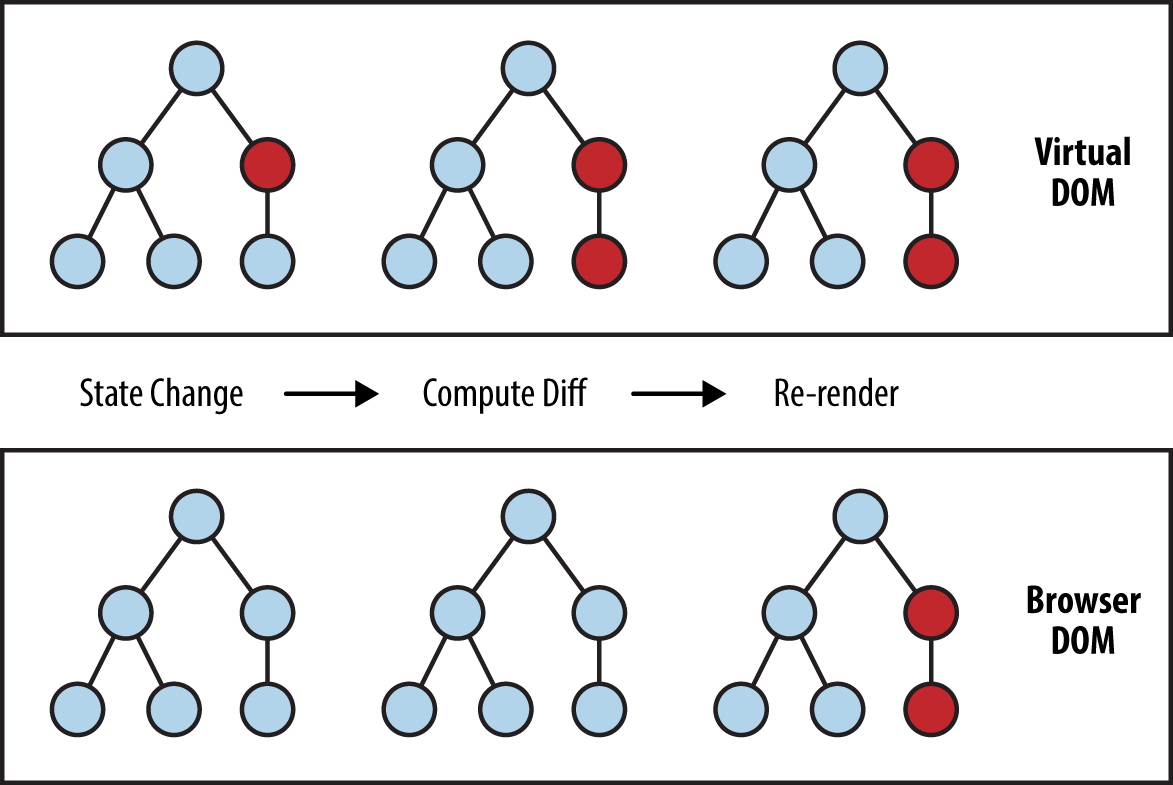
\includegraphics[width=0.8\textwidth]{images/cap4/react-virtual-dom.eps}
\caption[Funcionamiento del DOM virtual de React]{Funcionamiento del DOM virtual de React \protect\cite{ReactVirtualDOM}}
\label{fig:Funcionamiento del DOM virtual de React}
\end{center}
\end{figure}

\bigskip
React es ampliamente utilizada por muchas empresas gracias a su capacidad de integrarse con otras librerías. 
Por ejemplo Microsoft mantuvo parte de la página en jQuery mientras realizaba la integración de React.

\bigskip
Otro ejemplo de grandes empresas que hagan uso de esta librería son: AirBnB, Netflix, Wallmart…  \cite{ReactUsers}

\bigskip
Y muchas de ellas han contribuido al ecosistema de React, ya sea mediante guías de estilo, conjunto de componentes, patrones... \cite{ReactStyleGuide}

\bigskip
Además,la comunidad de usuarios es increíblemente activa, por ejemplo es común ver a Dan Abramov resolviendo dudas
en distintos sitios como \textit{Github} o \textit{Reddit}. Dan Abramov es el creador de Redux (una implementación de gestión de estados), desarrollador de la nueva implementación de 
React \textit{(react-fiber)}, empleado de Facebook, participante en muchas conferencias y además autor de 
múltiples herramientas como \textit{react-hot-loader}. 

\bigskip
Debido a todo lo anterior y a que además, React tiene una excelente integración con Typescript utilizando 
el formato .tsx, queda claro que es la mejor opción posible para esta aplicación. React es una librería 
desarrollada por Facebook para construir interfaces.
